\begin{chapabstract}
\small{
This introductory chapter gives the reader the required background to understand the context of this work. It is organized as follows.
\autoref{s:Gamma-Ray-Astronomy} discusses $\gamma$-ray astronomy and ground-based $\gamma$-ray imaging with Cherenkov telescopes. \autoref{s:CTA} introduces the Cherenkov Telescope Array Observatory (CTAO), the science goals, an overview of the telescope array, and its associated computing and software systems, including the Science Alert Generation System. Finally, it explores the scientific use cases of serendipitous discoveries and follow-up observations linked to the real-time detection of transient events. \autoref{s:gamma-ray-data-analysis} covers gamma-ray data analysis techniques, including the full field of view maximum likelihood and the aperture photometry. It also describes the Li\&Ma significance estimation method in the context of a reflected regions background estimation algorithm. Finally, \autoref{s:Gamma-Ray-Bursts} covers the study of $\gamma$-ray bursts, the transient phenomena this work is focused on.
}\\
\begin{center}
\noindent\makebox[0.8\linewidth]{\rule{0.66\paperwidth}{0.4pt}}
\end{center}
\vspace{1cm}
\end{chapabstract}
\section{Gamma-ray Astronomy}
\label{s:Gamma-Ray-Astronomy}
Gamma-ray astronomy studies the most energetic electromagnetic radiation in the universe, with energies ranging from a few hundred keV to several PeV. The $\gamma$ photons are produced by some of the universe's most extreme and violent processes, including supernovae, black holes, and neutron stars \cite{Fishman1995}. Another type of $\gamma$ radiation is Cosmic Rays. They are produced by accelerating charged particles, such as electrons or protons, to very high energies through various processes, including the collapse of massive stars, the acceleration of particles in magnetic fields, and the collision of particles in high-energy environments. Therefore, the study of gamma rays provides a unique window into the physics of these extreme environments.
Two main components dominate the $\gamma$-ray sky: known sources and the diffuse $\gamma$-ray background \cite{Ackermann2015}. Known sources are individual objects or phenomena that have been identified and studied in detail, such as active galactic nuclei (AGN), pulsars, and supernovae. These sources are relatively bright and can be easily detected by $\gamma$-ray telescopes \cite{Abdo2010}.
On the other hand, the diffuse $\gamma$-ray background is a faint and diffuse emission present throughout the entire $\gamma$-ray sky \cite{Ackermann2015}. This background emission is thought to be produced by the collective emission of many faint sources that are too faint to be detected individually \cite{Abdo2010}. It is also thought to be produced by the interaction of cosmic rays with the interstellar medium and by the decay of radioactive isotopes \cite{bulgarelli_2019}.
One of the main challenges in studying the $\gamma$-ray sky is the difficulty in separating the contribution of known sources from the diffuse background emission \cite{Ackermann2015}. This is because the background emission is much brighter than the individual sources, making it difficult to study them in detail \cite{Abdo2010}. In addition, $\gamma$-ray is background dominated since, among the detected events, hadrons are 1 thousand times more frequent than $\gamma$ photons.
The study of gamma rays has a long history, dating back to the discovery of cosmic rays by Victor Hess in 1912. However, it was not until the development of space-based instruments in the 1960s and 1970s that $\gamma$-ray astronomy became a mainstream field of study. One of the first satellite missions to significantly contribute to the field was the Gamma Ray Observatory (GRO), launched by NASA in 1991. GRO carried a suite of instruments designed to detect and measure gamma rays from various sources, including the Crab Nebula, the Cygnus X-1 binary system, and the Galactic Center \cite{mattox_et_al_1996}. In the decades since the launch of GRO, advances in detector technology and instrumentation have allowed for the development of increasingly sensitive $\gamma$-ray telescopes. The Swift Gamma-Ray Burst Mission, launched by NASA in 2004, is specifically designed to detect and study $\gamma$-ray bursts \cite{swift_2004}. The AGILE satellite, launched by the Italian Space Agency in 2007, is a multi-wavelength observatory with a $\gamma$-ray imager (GRID) on board. AGILE has made several important discoveries in $\gamma$-ray astronomy, including detecting $\gamma$-ray emissions from the Milky Way's central region and discovering a new class of $\gamma$-ray sources called \textit{microquasars} \cite{Tavani_2009}. The Fermi Gamma-ray Space Telescope was launched by NASA in 2008. Using its Large Area Telescope (LAT), it surveys the $\gamma$-ray sky and has discovered many new $\gamma$-ray sources, including active galactic nuclei, pulsars, and $\gamma$-ray bursts \cite{Abdo2010}. 
Space telescopes have been developed because $\gamma$-ray radiation is opaque to the Earth's atmosphere. However, space satellites can capture gamma rays up to a certain energy. For gamma rays with higher energies, the dimensions and density of the detector make it infeasible to launch them into orbit. In order to capture the most energetic $\gamma$-rays, ground-based telescopes use the earth's atmosphere as a detector. These telescopes, such as the Cherenkov Telescope Array (CTA), are designed to detect the secondary products of gamma rays as they interact with the atmosphere. The most common secondary product detected is Cherenkov radiation, but other products, such as muons, can also be observed. Ground-based telescopes provide an alternative approach to studying the high-energy gamma-ray spectrum, complementing the data obtained by satellite-based detectors. The atmospheric Cherenkov technique is one way to detect the $\gamma$-ray radiation that ground-based $\gamma$-ray telescopes can use. It works by detecting the faint flashes of blue light created when high-energy gamma rays collide with the upper atmosphere. The first generation of atmospheric Cherenkov telescopes (IACTs) was the Whipple 10m telescope, the HEGRA array, and the CAT telescope. These telescopes were followed by the current generation of IACTs, including the High Energy Stereoscopic System (H.E.S.S.) \cite{hess_2000}, the Major Atmospheric Gamma Imaging Cherenkov (MAGIC) telescopes \cite{magic_1999}, and the Very Energetic Radiation Imaging Telescope Array System (VERITAS) \cite{weekes2002very}. The CTA observatory currently under construction is the next generation of ground-based $\gamma$-ray telescopes. CTA will consist of two arrays of telescopes, one in the northern and one in the southern hemispheres, with a total of more than 60 telescopes. The telescopes will have a large field of view (FOV) and a sensitivity that is an order of magnitude better than current IACTs, making it possible to study $\gamma$-ray sources with unprecedented precision. \autoref{ss:telescope-array} gives more details on the telescope array configurations.

\subsection{Ground-Based Gamma-Ray Imaging with Cherenkov Telescopes}
\label{ss:iact}
Cherenkov telescopes are designed to detect the Cherenkov radiation produced when high-energy particles and radiation pass through the Earth's atmosphere. 
When gamma rays reach the Earth's atmosphere, they interact with it and produce cascades of subatomic particles and radiation. These cascades are also known as air or particle showers. The ultra-high energy particles in these showers can travel faster than light in the air, which creates a flash of blue and ultra-violet light (Cherenkov effect), similar to how a sonic boom is created by an aircraft exceeding the speed of sound. While the light is spread over a large area, the cascade only lasts a few billionths of a second \cite{ong2009gamma}.  Cherenkov telescopes are typically composed of large mirrors and disposed to form a detector array. The mirrors reflect the Cherenkov radiation, and the camera, typically composed of photomultiplier tubes or charged coupled devices, captures the signal. The shower produced by a $\gamma$-photon projects an approximately elliptical shape on the camera, which is analyzed to reconstruct the primary gamma ray's origin, energy, and direction. This process is shown in \autoref{f:cherenkov-imaging}.
\begin{figure}[ht] 
\centering
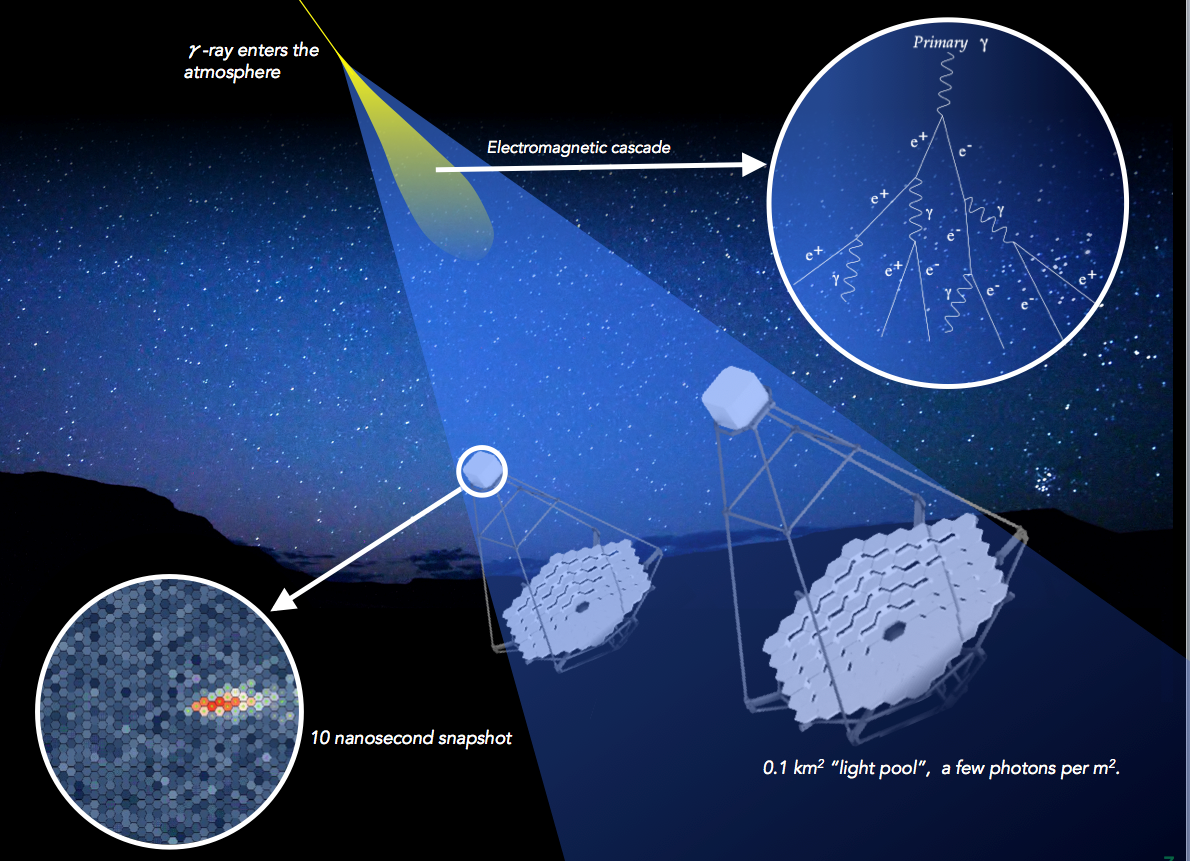
\includegraphics[width=1\textwidth]{figures/introduction/cherenkov-imaging.png}
\caption{Image explaining how Cherenkov Telescopes detect Cherenkov light produced by a primary $\gamma$-ray interacting with the Earth’s atmosphere. Credits to \cite{ctaobservatorywebsite}.}
\label{f:cherenkov-imaging}
\end{figure}
Electromagnetic showers, like those initiated by gamma rays, are different from hadronic showers initiated by cosmic rays (protons and nuclei) that have larger structures and can therefore be distinguished. The air showers initiated by electrons/positrons constitute an irreducible isotropic background for the telescopes. The efficiency in discriminating between hadronic and $\gamma$-ray showers defines, among other parameters, the telescope's minimum detectable flux or sensitivity \cite{tampieri2020real}. 
The flux quantity ($cm^{-2} s^{-1}$) describes how much light a source emits per unit of time and surface. The sensitivity is defined as the minimum flux value detectable with a confidence level of $5\sigma$. It depends on several parameters, such as the analysis algorithm, the observing conditions, the instrument response function, and the sub-array configuration. After the raw data is collected, an image-cleaning process occurs to reconstruct the shower information needed to perform the parametrization of the shower itself. A. M. Hillas introduced the fundamental image parameters in 1985 when a single telescope configuration was still used \cite{hillas1985cerenkov}. These parameters are:
\begin{itemize}
    \item Size: total number of photoelectrons in the shower image. It is proportional to the energy of the incoming primary $\gamma$-ray or particle;
    \item Length: is the half of the major axis of the shower image;
    \item Width: is the half of the minor axis of the shower image;
    \item Frac: measures the general concentration of light;
    \item Miss: is the perpendicular distance of the center of the field (where the source is supposed to be in a single telescope configuration and pointing in center of the field of view) from the image axis;
    \item Azimuthal-Width: is the image width relative to a new axis which
joins the center of the field to the centroid of the image; 
    \item Distance: is the distance of the brightest point from the center of the
field.
\end{itemize}
These parameters allow for evaluating the obtained Cherenkov images and achieving good $\gamma$-ray/hadron separation. 
New parameters are used to track the source position when the source is not in the camera center (see \autoref{sss:background-estimation}):
\begin{itemize}
    \item Alpha: is the angle between the major axis of the ellipse and the direction of the source position from the center of gravity of the image;
    \item Dist: is the distance of the center of gravity of the image from the source position.
\end{itemize}
\begin{figure}[ht] 
\centering
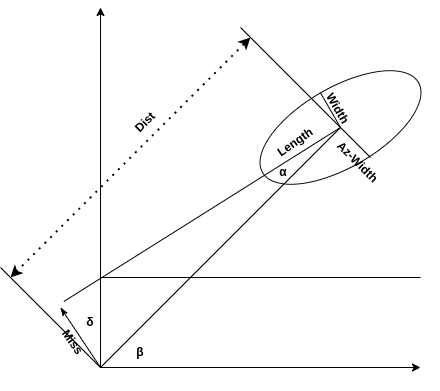
\includegraphics[width=0.7\textwidth]{figures/introduction/hillas.png}
\caption{Parametrization of a shower image through Hillas parameters.}
\label{f:hillas}
\end{figure}
\autoref{f:hillas} shows the Hillas parametrization of a shower image.
As we will see in \autoref{ss:telescope-array}, the CTA Observatory will use an array of Cherenkov telescopes to observe individual showers to reconstruct the three-dimensional origin of $\gamma$-ray showers. This technique, known as stereoscopic reconstruction, allows more effective reconstruction and discrimination of $\gamma$-ray showers from hadronic showers produced by isotropic cosmic rays. The stereo reconstruction increases the background suppression efficiency by about 100, improves the angular resolution, and enables morphological studies of extended $\gamma$-ray sources \cite{Spurio2018}.
These observations are analyzed using reconstruction algorithms based on Hillas’ parameters and implemented using statistical techniques like the Random Forest regression method \cite{Albert2008}. After the data is reconstructed, it is collected in the form of a photons list, i.e., a collection of individual photons along with their arrival time, reconstructed direction, and reconstructed energy. 

\section{The Cherenkov Telescope Array Observatory}
\label{s:CTA}
The CTA Observatory is a next-generation ground-based $\gamma$-ray observatory currently under development. CTA is a collaboration of over 1200 scientists from 32 countries and is expected to be the most sensitive and highest-resolution $\gamma$-ray observatory ever built \cite{ScienceWithCherenkovTelescopeArray2018}.

\subsection{Science goals}
\label{s:science-goals}
CTA will address a wide range of major questions in and beyond astrophysics. The Core Programme \cite{ScienceWithCherenkovTelescopeArray2018} provides a comprehensive discussion. In brief, the science goals can be grouped into three broad themes. 

The first theme is understanding the origin and role of relativistic cosmic particles. Relativistic particles play a significant role in many astrophysical systems, from pulsars and supernova remnants to active galactic nuclei and clusters of galaxies. However, the relationship between these particles, the turbulent motions of gas, and magnetic fields within our own galaxy and their overall impact on star formation and galaxy evolution is not well understood. CTA will provide the first high-resolution measurements of cosmic-ray protons and nuclei in astrophysical systems, giving insight into the processes of acceleration, transport, and feedback mechanisms. Historically, non-thermal effects in astrophysical systems have been ignored or approximated due to a lack of data. The insights from CTA will significantly contribute to our understanding of galaxy and cluster evolution in the era of precision astrophysics. The main goal of $\gamma$-ray astrophysics has been to identify where particle acceleration occurs and determine the main contributors to locally measured cosmic rays, mostly protons, and nuclei. Progress has been made in the last decade. Still, key questions remain unanswered, such as whether supernova remnants are the only major contributors to Galactic cosmic rays and the sources of high-energy cosmic electrons and ultra-high-energy cosmic rays. The question of how and where particles are accelerated in the universe is also important, as well as the role these particles play in the evolution of their host objects and how they are transported to large distances.

The second theme is about probing extreme environments. The acceleration of particles to extremely high energies is often linked to extreme environments, such as those found near neutron stars and black holes or in relativistic outflows or explosions. Very high-energy (VHE) emissions from these accelerated particles can serve as a probe of these environments, providing access to time and distance scales that are not accessible through other wavebands. VHE emission also often escapes from systems where UV and X-ray emission is absorbed, offering information independent of assumptions about magnetic field strengths. Furthermore, VHE photons from distant objects can probe the intervening space. CTA will allow us to measure the redshift evolution of the UV-IR background and, thus, the star-formation history of the universe and probe magnetic fields in cosmic voids at levels many orders of magnitude below the reach of any other technique. CTA will also determine if VHE photons heat the gas in these under-dense regions, potentially suppressing the formation of dwarf satellite galaxies.

The third theme is exploring frontiers in physics. CTA has the potential to make significant discoveries in the field of fundamental physics. CTA will reach the expected thermal relic cross-section for self-annihilating dark matter for a wide range of dark matter masses, including those inaccessible to the Large Hadron Collider. The long travel times of gamma rays from extragalactic sources, combined with their short wavelength, make them a sensitive probe for energy-dependent variations of the speed of light due to quantum-gravity-induced fluctuations of the metric. CTA will be sensitive to these effects on the expected characteristic scale, the Planck scale. Gamma rays may also couple to other light particles, such as axion-like particles (ALPs), under the influence of intergalactic magnetic fields, which effectively makes the universe more transparent to gamma rays and introduces a spectral modulation. Each of these effects would represent a major discovery and justify the effort of constructing and operating CTA. CTA's increased sensitivity and energy coverage bring these effects within reach and could allow for further discoveries in fundamental physics.


\subsection{The telescope array}
\label{ss:telescope-array}
CTA aims to capture the elusive cascades of $\gamma$-ray photons produced when high-energy gamma rays hit the Earth's atmosphere. These cascades are incredibly rare, with only one $\gamma$-ray photon per square meter per year from a bright source or one per square meter per century from a faint source. CTA will use more than 60 telescopes distributed between two array sites in the northern and southern hemispheres to improve the chances of capturing these elusive signals. The northern hemisphere array will have a more limited size and focus on the low and mid-energy range of CTA, between 20 GeV and 5 TeV. Meanwhile, the southern hemisphere array, which has a prime view of the rich central region of our galaxy, will cover the mid- to a high-energy range of CTA, spanning $\gamma$-ray energies from 150 GeV to 300 TeV \cite{Acharyya201935}. \autoref{fig:ctao-sens} shows the sensitivity of the northern and southern telescope arrays compared to other instruments. 
\begin{figure}[]
\centering
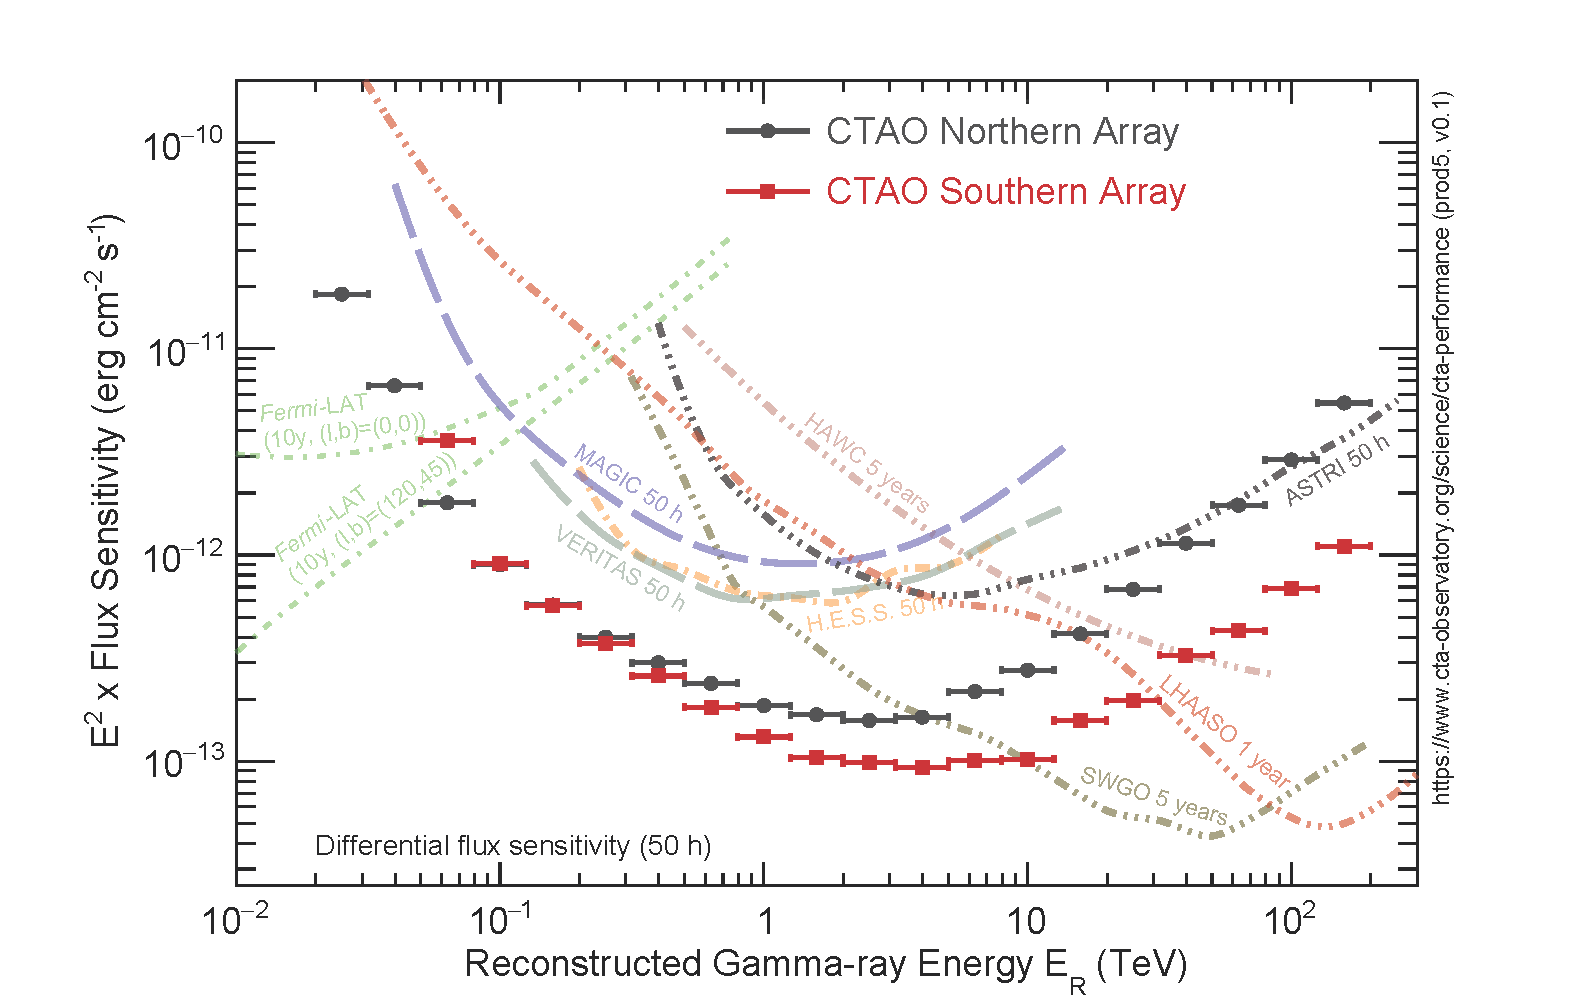
\includegraphics[width=1\linewidth]{figures/introduction/ctao-sensitivity.png}
\captionof{figure}{The sensitivity of the CTA Northern and Southern arrays compared to other instruments. Credits to \cite{zenodo_2021}}
\label{fig:ctao-sens}
\end{figure}
To cover the full CTA energy range, three classes of telescopes are required: Small-Sized Telescope (SST), Medium-Sized Telescope (MST), and Large-Sized Telescope (LST). The SSTs are the most sensitive to detect high-energy gamma rays and are therefore more suitable for the southern site's detection of higher-energy gamma rays. In the southern hemisphere, there is unobstructed visibility of the galactic center, which is a rich source of various types of emission. As a result, detecting low-energy gamma rays in this region is particularly challenging due to the high signal-to-noise ratio and the contribution of the diffuse background from the interstellar gas.  Scientists have conducted various simulations to determine the best configurations of arrays to maximize performance, including sub-array configurations. These configurations (shown in \autoref{fig:ctao-north} and \autoref{fig:ctao-south}) could allow for parallel and independent observations, resulting in optimized observation time and a more specific focus on science \cite{Acharyya201935}. The Alpha Configuration is the approved layout of the telescope arrays in both the northern and southern hemispheres. This configuration includes 13 telescopes, 4 LSTs, and 9 MSTs, distributed over an area of about $0.5 km^2$ in the CTA Northern Array and 51 telescopes over a $~3 km^2$ area, consisting of 14 MSTs and 37 SSTs, in the CTA Southern Array. The collaboration between the northern and southern hemispheres will allow CTA to expand its reach and study the universe in a more comprehensive way \cite{Acharyya201935}. 
\begin{figure}[ht]
\centering
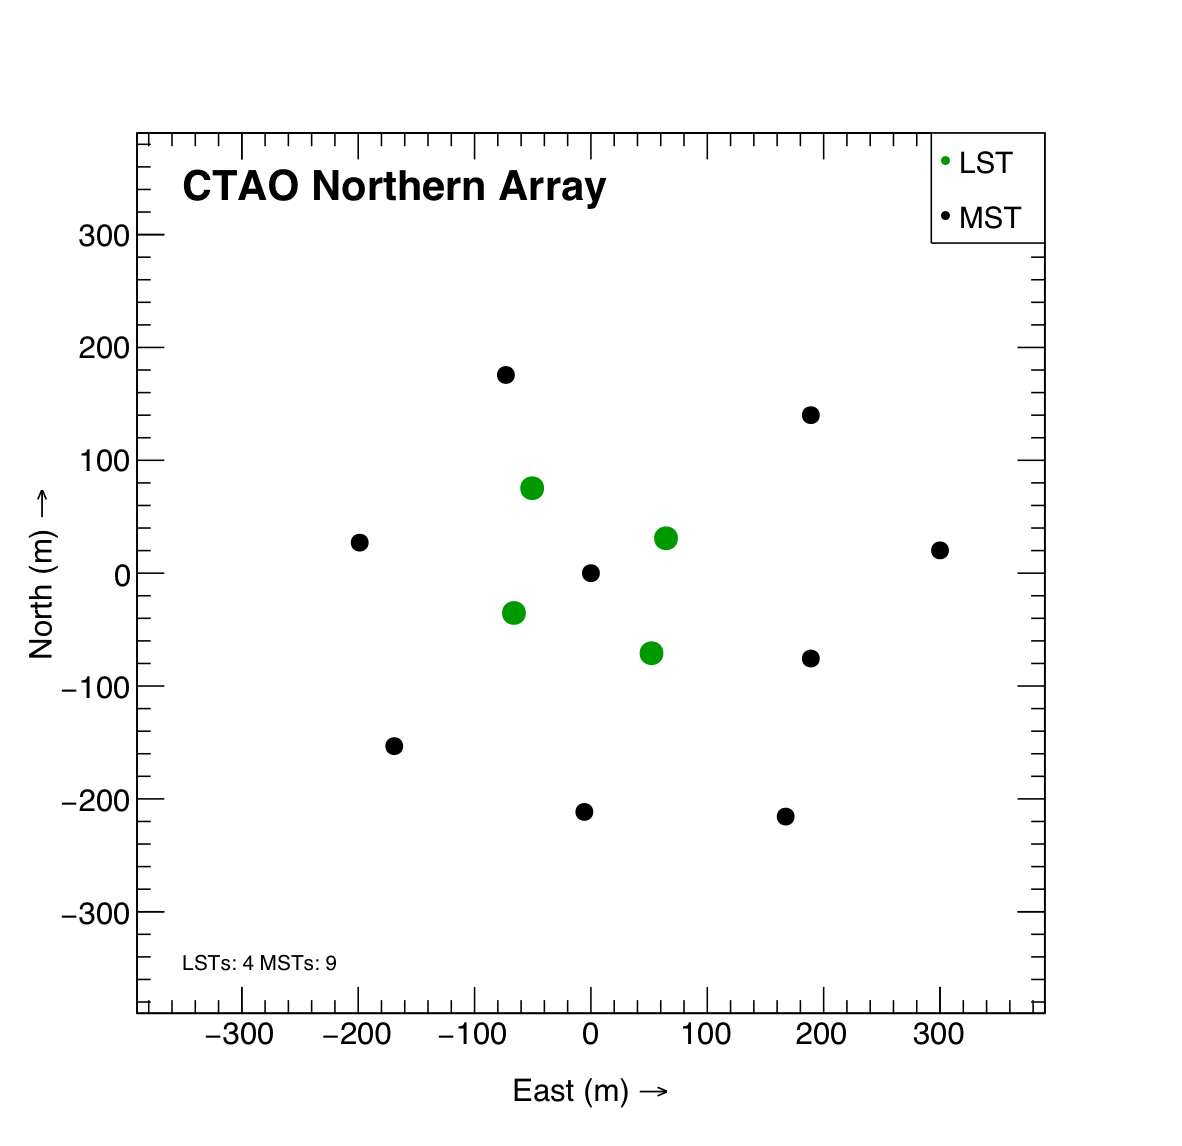
\includegraphics[width=0.8\linewidth]{figures/introduction/ctao-north.png}
\captionof{figure}{Layout of the CTA Northern array on La Palma (Spain), including the elements defined in the Alpha Configuration. Credits to \cite{zenodo_2021}}
\label{fig:ctao-north}
\end{figure}
\begin{figure}[ht]
\centering
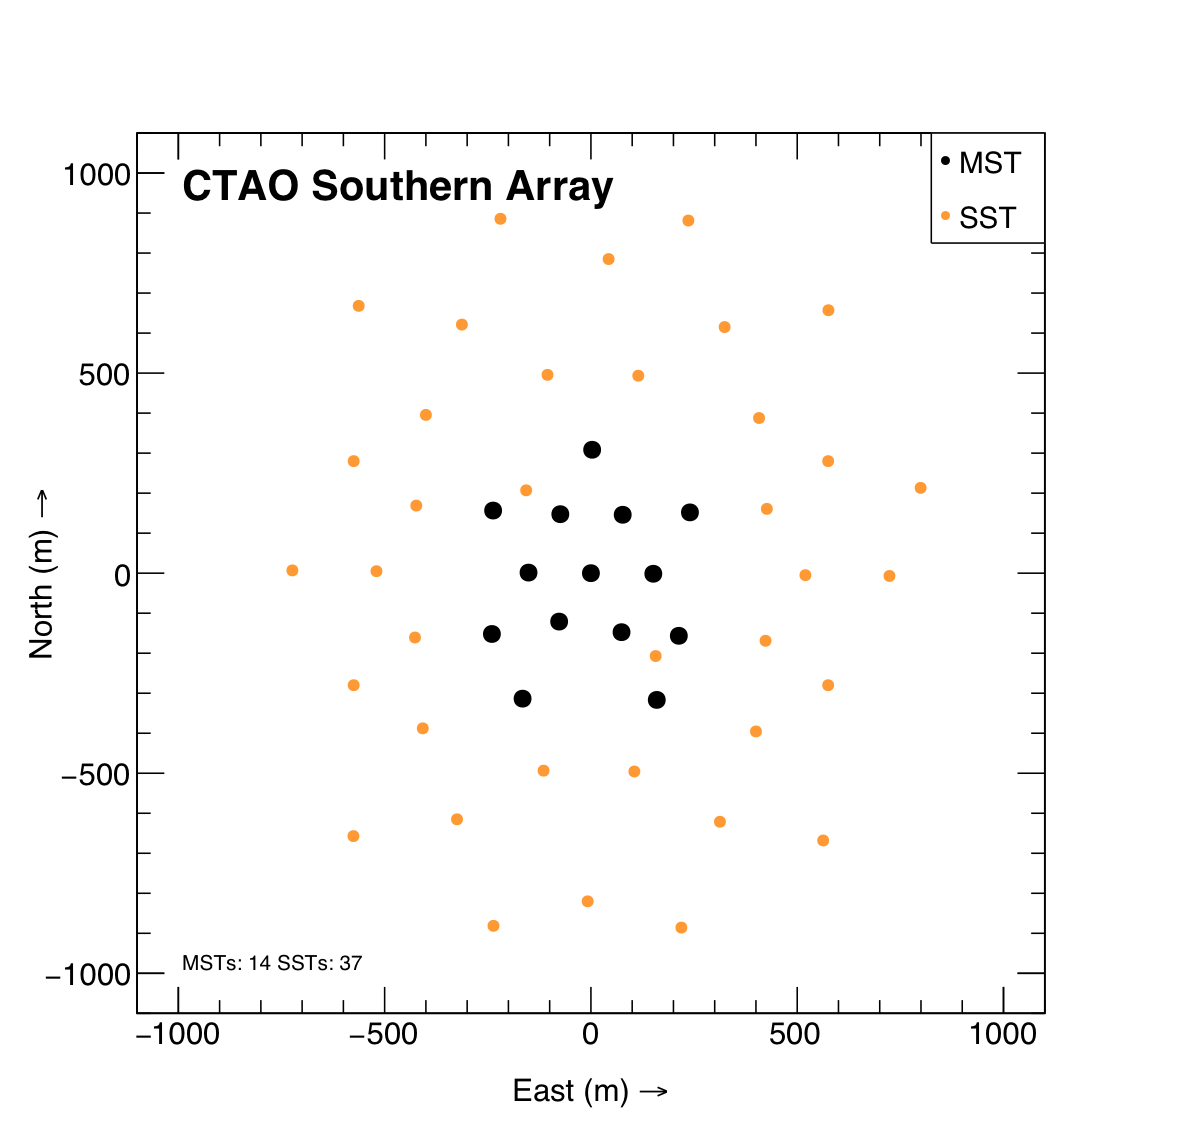
\includegraphics[width=0.8\linewidth]{figures/introduction/ctao-south.png}
\caption{Layout of the CTA Southern array in the Atacama Desert (Chile), according to the Alpha Configuration. Credits to \cite{zenodo_2021}}
\label{fig:ctao-south}
\end{figure}
The northern hemisphere array will be located at the existing site of the Instituto de Astrofisica de Canarias' (IAC's) Observatorio del Roque de Los Muchachos on the island of La Palma in the Canary Islands. This site already hosts an operating $\gamma$-ray observatory, the Major Atmospheric Gamma Ray Imaging Cherenkov (MAGIC) telescopes, and various optical telescopes of various sizes. The Southern Hemisphere Array will be located in the Atacama Desert in Chile, near the European Southern Observatory's (ESO's) existing Paranal Observatory. 

\subsubsection{Large-Sized Telescopes (LST)}
\begin{figure}[t]
\centering
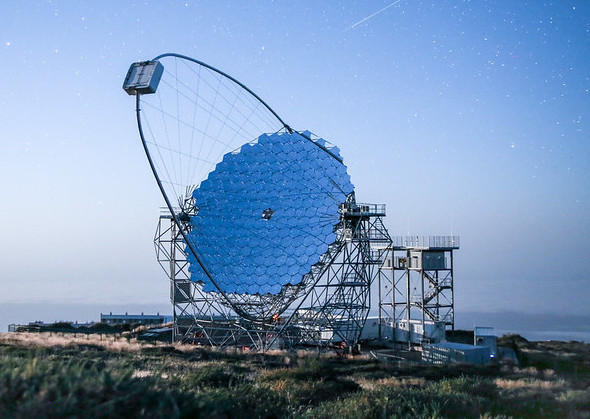
\includegraphics[width=0.9\linewidth]{figures/introduction/lst.jpg}
\caption{The LST Prototype, LST-1, on the CTA-North site in La Palma. Credits to \url{https://www.flickr.com/photos/cta_observatory/albums/72157671493684827}} 
\label{fig:lst}
\end{figure}
This section describes the Large-Sized Telescope (LST) referring \cite{Barrio_2020} and \cite{ctaobservatorywebsitetechnology}.
The LST project is a collaboration involving over 100 scientists from 10 countries, including Brazil, Croatia, France, Germany, India, Italy, Japan, Poland, Spain, and Sweden. The LST is designed to capture images of low-energy gamma rays, which produce a small amount of Cherenkov light. The LST uses a large mirror with a $23m$ diameter parabolic reflective surface supported by a tubular structure made of reinforced carbon fiber and steel tubes (\autoref{fig:lst}). Four LSTs will be placed at the center of the northern hemisphere array to capture low energy sensitivity of CTA between 20 and 150 GeV. The LSTs also have a very good sensitivity up to energies of a few TeV, which is, however, more efficiently covered by Medium-Sized Telescopes (MSTs). The LST is an alt-azimuth telescope that uses a reflective surface of 400 squared-meters to collect and focus the Cherenkov light into the camera. The camera comprises photomultiplier tubes that convert the light into electrical signals that dedicated electronics can process. Although the LST is 45 meters tall and weighs around 100 tonnes, it is designed to be extremely nimble and able to re-position within 20 seconds. This re-positioning speed and low energy threshold are critical for CTA studies of galactic transients, high red-shift active galactic nuclei, and $\gamma$-ray bursts. The LSTs will also expand the science reach to cosmological distances and fainter sources with soft energy spectra. 
The LST Camera shares many elements with the NectarCAM for the MSTs. The camera has a total field of view of about 4.3 degrees and is designed to be compact and lightweight while providing optimal performance at low energies. Each pixel incorporates a photosensor and the corresponding readout electronics. These electronics are based on the Domino Ring Sampler Version 4 (DRS4) chip, developed at the Paul Scherrer Institute in Switzerland and currently used by several experiments, including the MAGIC Cherenkov telescopes. The camera trigger strategy is based on the shower topology and the temporal evolution of the Cherenkov signal produced in the camera. The LST prototype, LST-1, was completed in October 2018 in La Palma, Canary Islands, Spain, on the site of the Observatorio del Roque de Los Muchachos. The prototype is foreseen to become the first LST telescope of CTA and, in fact, the first telescope on a CTA site to be operated by the observatory. It will need to undergo a critical design review to verify that the design complies with CTA science goals, operational needs, safety standards, etc. before CTA formally accepts it.
On October 10th, 2018, over 200 guests from around the world gathered to celebrate the inauguration of the prototype Large-Sized Telescope (LST-1). On December 14th, 2018, the LST-1 prototype recorded its first Cherenkov light. On November 23rd, 2019, LST-1 successfully detected its first $\gamma$-ray signal when pointing to the Crab Nebula. Between January and February 2020, the LST-1 prototype observed the Crab Pulsar, a neutron star at the center of the Crab Nebula. These observations were used to verify the telescope's performance and capabilities.

\subsubsection{Medium-Sized Telescopes (MST)}
\begin{figure}[t]
\centering
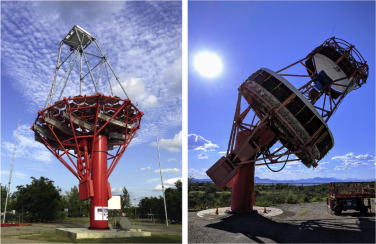
\includegraphics[width=0.9\linewidth]{figures/introduction/mst.jpg}
\caption{The MST design explores two different concepts. On the one hand, inspired by HESS and VERITAS current observatories, a 12 meters diameter modified Davis–Cotton (DC-MST) optical layout and a PMT camera. On the other, a novel 10 meters diameter Schwarzschild–Couder (SC-MST) optics incorporating a novel Silicon Photo-Multiplier (SiPM) camera. Credits to \cite{Barrio_2020}.} 
\label{fig:mst}
\end{figure}
This section describes the Medium-Sized Telescope (MST) referring \cite{Barrio_2020} and \cite{ctaobservatorywebsitetechnology}.
An international team of institutes and universities from Austria, Germany, France, Brazil, Poland, Spain, Switzerland, and Italy is developing the Medium-Sized Telescope (MST). This telescope is considered the \textit{workhorse} of the CTA, with sensitivity in the core energy range of CTA, from about 150 GeV to 5 TeV. The CTA plans to include 23 MSTs, with 14 in the southern and 9 in the northern hemispheres. The MST mirror will be about 12 meters in diameter and have two camera designs using photomultiplier tubes (PMTs).
The MST is a modified Davies-Cotton telescope with a reflector diameter of 12 meters on a polar mount and a focal length of 16 meters. To create a uniform reflector, the MST will have up to 90 hexagonal-shaped mirrors aligned with an active mirror control assembly. The MST cameras will have a large field of view of about 8 degrees, making it easier to observe $\gamma$-ray sources that may be concentrated in one area of the sky or widely spread apart. Two camera concepts are in development for the MST: NectarCAM and FlashCAM. NectarCAM uses the ‘Nectar’ analog pipeline ASIC for signal capture with GSample/s sampling rate and shares many design features/components with the LST camera. NectarCAM is composed of 265 individual and easily removable modules. FlashCAM design follows a horizontal architecture with the photon detector plane (PDP), the readout electronics (ROS), and the data acquisition system (DAQ) as key building blocks. The PDP contains photomultiplier tubes (PMTs) arranged in a hexagonal structure.
An MST prototype was deployed in Berlin in 2012 and is currently undergoing performance testing. The main purpose of the prototype is to validate the design of the individual components, test the interfaces between the mating assemblies, and define the assembly process of the product. The prototype has a fully functional drive system, cameras for pointing and tracking, sensors designed to record the behavior response of the structure and drive system, and a weather station. The prototype is a fully-functioning telescope but doesn't include the entire camera assembly and its readout. Camera demonstrators were built, tested, and validated in parallel by the two camera sub-projects.

\subsubsection{Small-Sized Telescopes (SST)}
\begin{figure}[t]
\centering
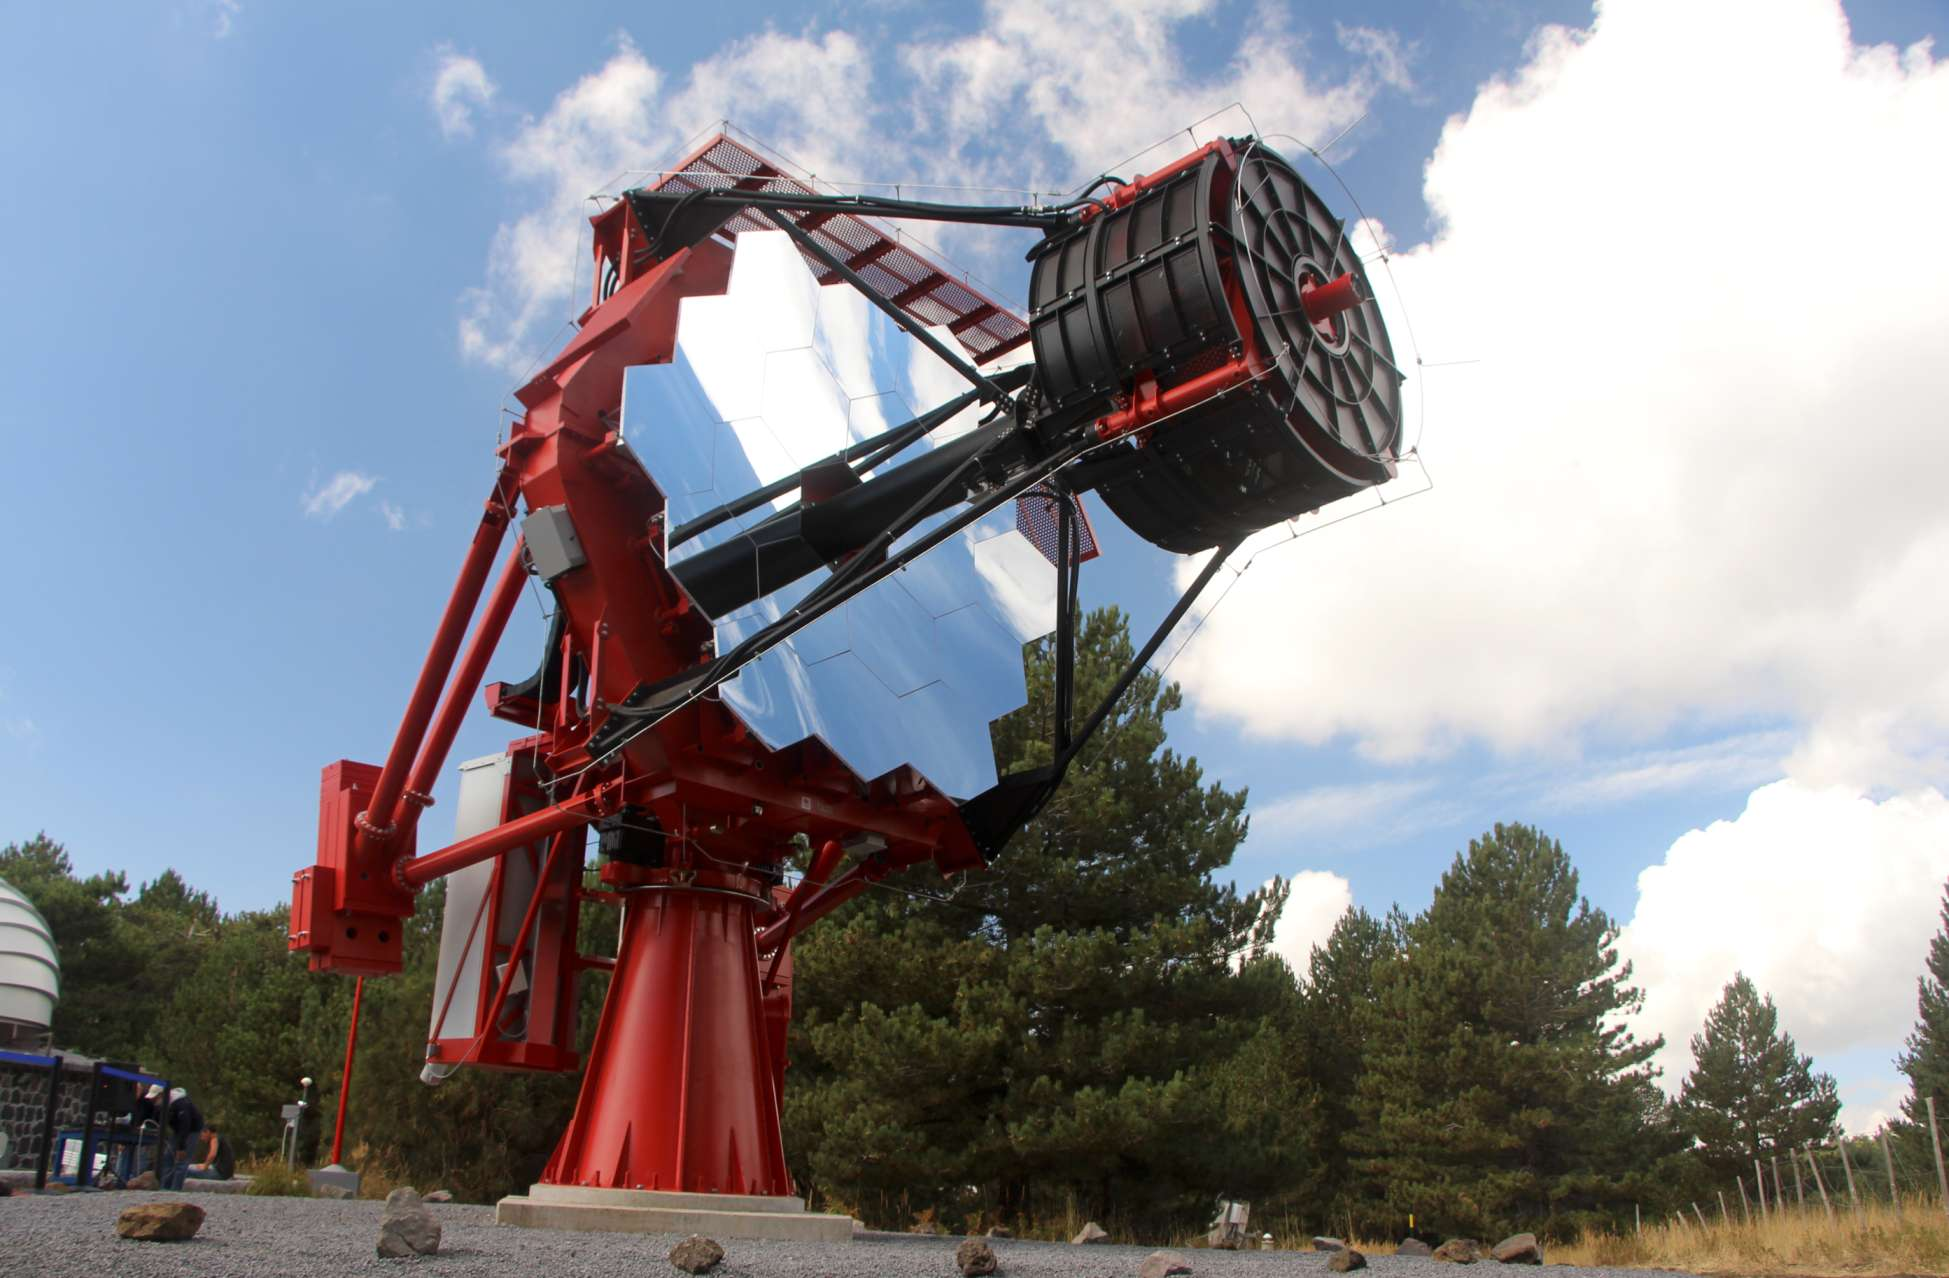
\includegraphics[width=0.9\linewidth]{figures/introduction/sst.jpg}
\caption{The ASTRI telescope prototype, a novel dual-mirror Schwarzschild-Couder telescope design proposed for the CTA. Credits to \cite{ctaobservatorywebsite}} 
\label{fig:sst}
\end{figure}
This section describes the Small-Sized Telescope (SST) referring \cite{Tagliaferri_2022} and \cite{ctaobservatorywebsitetechnology}.
The Small-Sized Telescopes will make up the largest number of telescopes in the CTA, with 37 planned to be spread out over several square kilometers in the southern hemisphere array only. This is because very high-energy $\gamma$-ray showers produce a large amount of Cherenkov light over a large area. The SST's smaller mirror is sensitive to the highest energy gamma rays (between a few TeV and 300 TeV). The SSTs wide coverage and high sensitivity improve CTA's chances of detecting the highest energy gamma rays. Three different SST implementations were proposed for the final SST design: ASTRI-Horn, GCT, and SST-1M. In 2018, a harmonization process was initiated. In June 2019, the council accepted the CTA Management proposal, stating that \textit{the CTA-SST design should be based on the ASTRI/CHEC design, taking into account the experience gained from all designs}. The SST design is a dual-mirror Schwarzschild-Couder aplanatic configuration, and thanks to its small plate scale, it uses a novel compact camera based on SiPM sensors. The 4.3m diameter primary mirror is segmented into hexagonal facets, and the 1.8m secondary mirror is monolithic. The SST's camera, also known as the CHEC camera, uses custom peak-hold application-specific integrated circuits (ASICs) for signal capture. The dual-mirror design allows for the same angular resolution and collecting area across a wide field of view with a short focal length. The camera comprises 2048 silicon photo-multiplier pixels forming approximately a 9x9 degrees field of view. The CHEC is unique as an SST dual-mirror camera in its ability to capture Cherenkov light not as fixed images but as movies consisting of hundreds of frames, each lasting one billionth of a second. The SST collaboration benefits from the research and development work previously carried out within the ASTRI, CHEC, and GCT projects to develop end-to-end SST dual-mirror telescopes. The ASTRI project is led by the Italian National Institute of Astrophysics (INAF) with the collaboration of several Italian universities, the Italian National Institute of Nuclear Physics (INFN), Universidade de São Paulo in Brazil, and North-West University in South Africa. 
The ASTRI project designed and installed an end-to-end dual-mirror prototype of the CTA small-size telescope (SST) on Mt. Etna (Sicily) and will install a dual-mirror SST mini-array composed of nine units at the CTA Southern site.
The ASTRI mini-array will extend the current IACTs sensitivity well above a few tens of TeV \cite{Vercellone_2016}. The CHEC project, led by MPIK, is an international collaboration between the University of Adelaide, the University of Amsterdam, DESY Zeuthen, Durham University, the Erlangen Centre for Astroparticle Physics (ECAP), the University of Leicester, the University of Liverpool, Nagoya University, and the University of Oxford. The Observatoire de Paris-Meudon carries out the GCT telescope project.

\subsection{Computing and software}
The CTA Computing Department faces the challenge of designing and implementing a system that supports all aspects of the CTA Observatory, from accepting observation proposals to scheduling observations, controlling the telescopes, processing and archiving data, and making it accessible to the public using open standards and FAIR (findability, accessibility, interoperability, and reusability) principles. The department is responsible for all stages of development, from architectural design to construction, validation, deployment, and maintenance. The Observatory's technical challenges and long lifetime will require new techniques and technologies to meet scientific demands. Even when built, maintaining the software and hardware systems for the 30-year lifespan of the observatory and the science data archive for an additional 10 years will not be a simple task. Therefore, software systems engineering is just as crucial as the code itself \cite{Oya2017}. In addition, the CTA array sites will generate a vast amount of data from the telescopes in hundreds of petabytes annually. This data will then be compressed and reduced to a few petabytes per year before being transferred to off-site data centers for processing and storage. Additionally, tens of petabytes of simulated data will also be generated and processed.
\begin{figure}[ht]
\centering
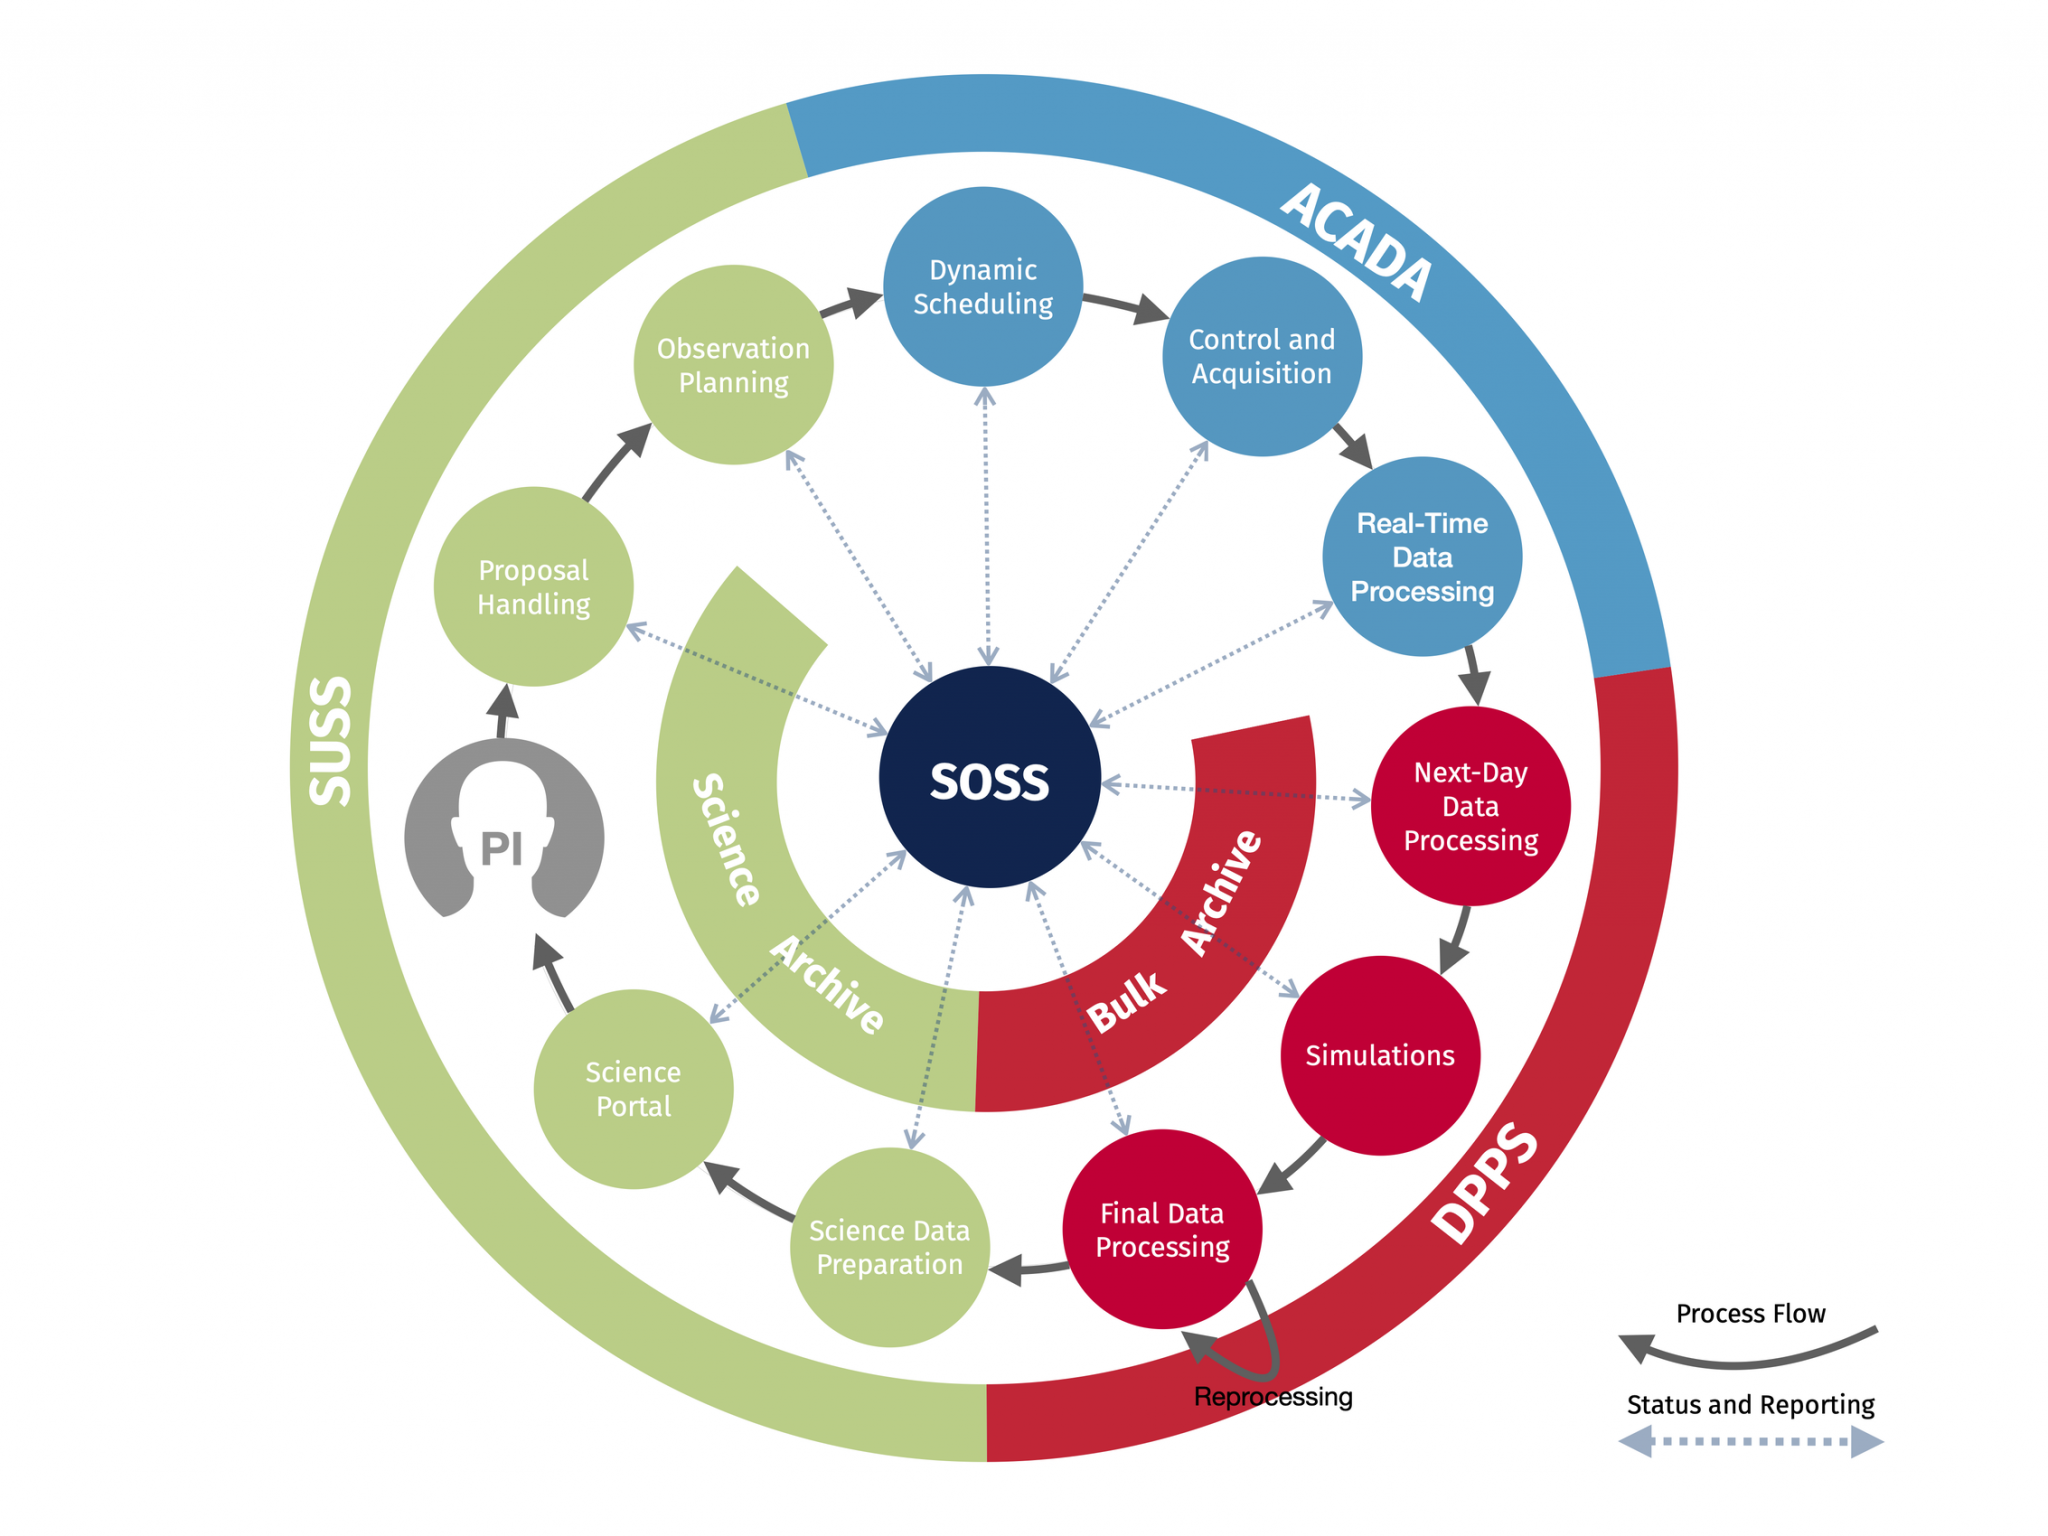
\includegraphics[width=0.9\linewidth]{figures/introduction/cta-softwares.png}
\caption{The diagram below provides a general overview of how the software systems interact with the main processes involved in the science operations of the observatory, including the submission, execution, and return of processed data related to a scientific proposal. Credits to \cite{ctaobservatorywebsitetechnology}.}
\label{fig:cta-softwares}
\end{figure}
The software systems that will satisfy all the CTA requirements are shown in \autoref{fig:cta-softwares}: the Array Control and Data Acquisition System (ACADA), the Data Processing and Preservation System (DPPS), the Science User Support System (SUSS), and the Science Operations Support System (SOSS) \cite{ctaobservatorywebsitetechnology}. 
The ACADA (Acquisition and Control and Data Analysis) system manages the supervision and control of telescopes and calibration instruments at both CTA array sites, including the efficient execution of scheduled and dynamically triggered observations. It also manages raw data acquisition and compression and generates automatic science alerts. The ACADA provides a user interface for site operators and astronomers \cite{Oya2017}. It's composed of several subsystems such as the Resource Manager and Central Control system \cite{Melkumyan2019}, the Human Machine Interface system \cite{Sadeh2017}, the Short-Term Scheduler system \cite{Colome2014}, and the Science Alert Generation Pipeline \cite{Bulgarelli2014}. The latter allows the observatory to reconstruct and analyze the data, detect sources, and issue candidate science alerts in real-time. As we will see later, this system is the context in which this work has been carried out. The DPPS (Data Processing and Preservation System) is responsible for transforming the raw data products generated by ACADA into low-level science data products suitable for analysis, which are then delivered to the SUSS (Science User Support System) for dissemination. The DPPS ensures that all data products are preserved and replicated in at least two off-site data centers, have traceable and reproducible provenance, and are of the highest scientific quality. It also provides continuous monitoring and quality reporting for its sub-systems and produces high-level science quality metrics and reports related to the services provided. The DPPS is implemented as a distributed system, deployed as a set of Data Processing and Preservation Nodes, running at the CTA-North and CTA-South data centers, on three CTA off-site data centers, and at the SDMC Data Center \cite{ctaobservatorywebsite}. The SUSS manages the software system for high-level science operations workflows, from proposals to data delivery and user support. It is the main access point for exchanging science-related products with science users. It provides software for observation planning, the automatic generation and verification of high-level science data products, the Science Archive, Science Analysis Tools, and Science Portal, which provides access to software applications, services, data, and software products \cite{Oya2017}. The SOSS (Science Operations Support System) is a collection of software tools that support the systems involved in science operations workflows, such as ACADA, DPPS, and SUSS \cite{ctaobservatorywebsite}. The respective systems can access and share science operations-related information and configurations. It includes the means to track the state of proposals and observations throughout their life cycle and the state of the CTA Observatory throughout the science operations workflow and science performance.


\subsection{The Science Alert Generation System}
\label{s:sag}
As described in \cite{bulgarelli2015on} and \cite{Bulgarelli_2021}, the Science Alert Generation system will perform real-time scientific analysis to issue science alerts. A science alert is a notification within the astrophysics community to share information about a transient phenomenon (such as an AGN's $\gamma$-ray flare, $\gamma$-ray bursts, gravitational waves, or galactic transients) that has been observed. Sharing this information through specialized communication networks allows coordination among different observatories to enable multi-wavelength and multi-messenger analysis. Those are rapidly developing fields that study celestial objects and phenomena using a wide range of electromagnetic and non-electromagnetic signals. This includes everything from radio waves and visible light to gamma rays, gravitational waves, and particles, such as cosmic rays and neutrinos. One of the key advantages of multi-wavelength and multi-messenger astronomy is that it allows astronomers to study the universe from a more comprehensive perspective. By combining data from different wavelengths and messengers, astronomers can better understand the physical processes in the universe. One of the most significant developments in multi-wavelength and multi-messenger astronomy has been detecting gravitational waves, ripples in space-time predicted by Einstein's theory of general relativity. The acceleration of massive objects, such as the merging of binary black holes or neutron stars, produces these waves. The first gravitational wave detection was made in 2015 by the Laser Interferometer Gravitational-Wave Observatory (LIGO) \cite{gw_061102}. Since then, several other gravitational wave detections have been made, opening up a new window onto the universe \cite{abbott2016observation}. The Science Alert Generation system will have a key role in the GW follow-up program \cite{seglar2019gravitational}. Another important aspect of multi-wavelength and multi-messenger astronomy is the study of transient phenomena, such as supernovae, $\gamma$-ray bursts, and fast radio bursts. These events are often brief and elusive and can be studied more effectively by combining data from multiple telescopes and instruments. For example, the combination of data from X-ray, optical, and radio telescopes has allowed for the study of the afterglows of $\gamma$-ray bursts (GRBs), which are thought to be the result of the collapse of massive stars or the merging of binary neutron stars \cite{Fishman1995}.
To achieve collaboration between observatories, the transient phenomena must be observed in real-time on a short timescale. Furthermore, if an external observatory identifies a transient, it is essential to react quickly, change the pointing of the telescopes, and analyze the data in an automated and fast way to confirm the transient event and to conduct follow-up observations \cite{Bulgarelli_2021}. 
\subsubsection{Requirements}
\label{ss:sag-requirements}
Technical challenges, such as limited network bandwidth at the observatory sites and a high expected data rate, make it difficult to perform real-time analysis off-site. As a result, an on-site analysis pipeline is necessary to access raw data, perform calibration, and produce scientific results \cite{bulgarelli2015on}. The real-time analysis must meet challenging requirements to process the large amount of data produced by CTA in real-time. The Science Alert Generation system must be able to generate candidate science alerts within 20 seconds from the last acquired event, with a maximum telescope positioning time of 90 seconds in response to external or internal triggers. These candidate science alerts will be sent to the Transients Handler system, which will evaluate the results of the SAG to generate the final science alert to the community within 5 seconds of receiving it. If we also consider the 5 seconds required to acquire data, CTA will be capable of issuing science alerts with a maximum latency of 30 seconds \cite{Bulgarelli_2021}.
Furthermore, the SAG system must be available during observations for at least 95\% of the time to enable real-time follow-up of external alerts and internal alerts triggering serendipitous discoveries. This will require re-scheduling observations to follow up the phenomena in real-time and maximize the coordinated outcome of the facilities' network \cite{di2020detection}. According to the CTA design requirements, the real-time search for transient events should be performed on multiple time scales (from minutes to hours) with a sensitivity not worse than two times the nominal CTA sensitivity. 
\cite{fioretti2015real} performed a preliminary evaluation of the real-time analysis sensitivity as a function of the CTA high-level technical performance (e.g., effective area, point spread function) and the observing time. 
 
\subsection{The scientific use cases}
\label{s:contribution-1-use-cases}
The growing interest in multi-messenger and multi-wavelength astronomy has greatly enhanced the search for transients. As stated in \autoref{s:science-goals}, the KSP for transients plans to invest a significant amount of observation time per year (\autoref{fig:transient-schedule}). The main source classes targeted by this KSP are Gamma-Ray Bursts (GRBs), Galactic transients, X-ray, optical, and radio transients, High-energy neutrino transients, GW transients, and serendipitous VHE transients \cite{ScienceWithCherenkovTelescopeArray2018}. GRBs are expected to be a major component of this KSP and will be detected based on external alerts (covered in \autoref{s:follow-up-observation}), but with the possibility of serendipitous discoveries (covered in \autoref{s:serendipitous-discoveries}).
\begin{figure}[t]
\centering
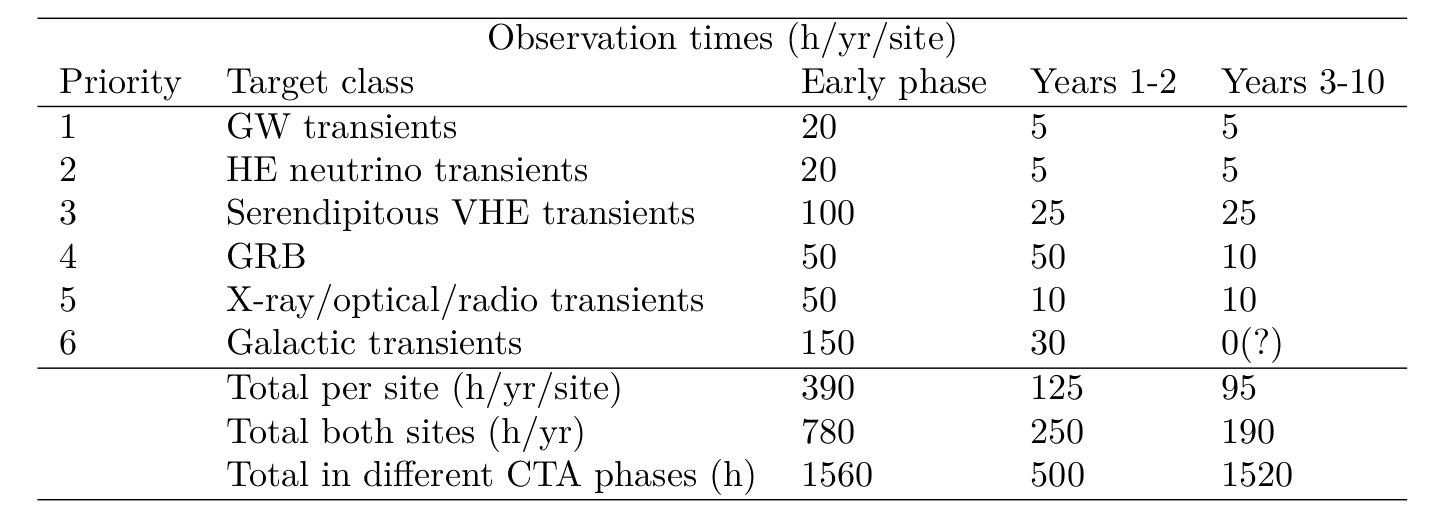
\includegraphics[width=0.9\linewidth]{figures/introduction/transients-schedule.png}
\caption{Maximum observation times required for follow-up targets in the Transient KSP, taken from. Credits to \cite{di2020detection}}
\label{fig:transient-schedule}
\end{figure}

\subsubsection{Serendipitous discoveries}
\label{s:serendipitous-discoveries}
Serendipitous discoveries are unexpected findings made while studying a specific target or phenomenon. This can happen because the telescope's field of view is larger than the region of interest used to observe a particular source. Large fields of view enable the detection of signals from multiple sources simultaneously. However, the probability of a serendipitous GRB event appearing in the field of view during an observation is very low. During the survey phases of CTA, large regions of the sky will be systematically observed, increasing the probability of serendipitous discoveries. The event must be detected as soon as possible to broadcast a science alert to other observatories to follow the same event and enable multi-wavelength and multi-messenger analysis \cite{bulgarelli2015on}. 

\subsubsection{Follow-up observation triggered by an external science alert}
\label{s:follow-up-observation}
Follow-up observations refer to a strategy of observing a specific target or phenomenon in more detail after an initial discovery or detection. The follow-up observations can be triggered by a science alert, which is a notification that alerts researchers and facilities of an interesting or unusual event happening. Follow-up observations can be conducted using various instruments and techniques. They are typically performed to study a target in more detail, confirm an initial discovery, and gather additional information about the target's properties \cite{ScienceWithCherenkovTelescopeArray2018}. When a science alert is received, the observatory will interrupt the current observation and will point to a new sky region to detect the new source in the least possible time. IF the error on the source's position is bigger than the field of view of the telescopes,  multiple follow-up observations with a tiling strategy \cite{bulgarelli2015on} are required to cover the whole localization region. In addition, the event's evolution cannot be observed from the beginning due to the delay between detecting the source that triggered the science alert, the time to receive it, and the time the telescopes took to change their pointing to the new sky region. 



\section{Analysis of Gamma-ray data}
\label{s:gamma-ray-data-analysis}
As outlined in \autoref{ss:iact}, when a high-energy photon from a $\gamma$-ray source collides with the Earth's atmosphere, it produces an electromagnetic air shower that results in Cherenkov emission, which is then observed with an optical telescope on the ground. The light from the shower triggers the telescope, and the incoming signals are processed and classified to reconstruct the primary event's energy and arrival direction. However, observations are heavily affected by background events caused mainly by cosmic hadrons, so significant effort is required to differentiate between electromagnetic events and background noise. The reconstruction outcome is a photon list, a collection of individual photons along with their arrival time, reconstructed direction, and reconstructed energy. The high-level $\gamma$-ray analysis is carried out at this stage to generate skymaps, spectra, and light curves and finally perform detections. This section will discuss the Aperture Photometry and Full-FOV Maximum Likelihood and  techniques. The \textit{Li\&Ma} significance estimation method is also described in the context of a \textit{reflected regions} background estimation algorithm. Their usage in the real-time scenario has been investigated by \cite{tampieri2020real}, \cite{di2020detection}, and \cite{di2021detection}. 

\subsection{The calibration database and the Instrument Response Functions}
\label{ss:caldb}
The calibration database contains \textit{instrument response functions}, required to simulate and analyze CTA event data. The instrument response function (IRF) $R(\bm{p}',E',t'|\bm{p}, E, t)$ describes the transformation from the physical properties of a photon (sky direction $\bm{p}$, energy E, and time t) to the measured characteristics of an event $\bm{p'},E',t'$ (the instrument response function is given in units of $cm^2 sr^{-1} s^{-1} MeV^{-1}$) \cite{Knodlseder_2016}. 
The IRF can be factorized in \textit{effective area} $A_{eff}(\bm{p},E,t)$ in the units of $cm^2$, \textit{point-spread function} $PSF(\bm{p}|p,E,t)$, and \textit{energy dispersion} $E_{disp}(E'|\bm{p},E,t)$. Furthermore, every IRF includes an account of the background rates as they vary in relation to energy and location within the field of view. The background rate mostly comprises cosmic-ray hadrons and electrons that pass the gamma-ray selection criteria (cuts) \cite{di2020detection}. During a simulation, the response of the instrument is applied to the ideal simulation model  to obtain the data as it was seen by the telescope. Instead, the telescope observation data must be restored during the analysis to obtain the real quantities, considering the IRF.


\subsection{Aperture photometry}
\label{ss:aperture-photometry}
Aperture photometry is a method to determine the number of photons recorded in a region of interest called the \textit{on region} and compare it to an estimate of the residual cosmic-ray background. This estimate is scaled appropriately before the comparison \cite{mohrmann2019}. The on/off method is applied to a list of photons to estimate the source event counts. The method consists in defining an aperture, a closed region centered on the source, to count the on-source photons. The background is estimated by observing one or more off-source regions with no source signals. The number of photons in these regions is the background contribution. To minimize the impact of background contamination and nearby sources on the data analysis, it is important to carefully select the regions used for the on-region and off-region. Ideally, the on-region should be chosen so as to contain the point spread function of the instrument at the given energy range, while the off-region should be of equal size and chosen in a way that minimizes the contamination of background or nearby sources. This ensures that the counts in the on-region are not underestimated or overestimated, providing a more accurate measurement of the gamma-ray source of interest. Still, it is also important to ensure that the background regions share similar characteristics with the source, including the instrument response function in that region. To determine the number of excess photons from the source, the normalized number of off-region events is subtracted from the on-region data. If the on-region and off-region share the same size, offset, and exposure time, the probable number of photons contributed by the source is calculated using the following formula:
\begin{equation}
NS = N_{on} - \alpha*N_{off}
\end{equation}
where $N_{on}$ are the counts in the source region, $N_{off}$ are the counts in the background regions, and $\alpha$ is a background scale factor.
To obtain valid background statistics, it is usually necessary to take multiple observations, which introduces additional scaling factors to consider. These factors include the effective areas, exposure, and region size between the on and off observations. With the counts in the on and off regions, and the excess counts, it is possible to estimate the detection significance and the source flux in a simple and fast way without the need for modeling \cite{tampieri2020real}. A light curve can be constructed by aligning multiple flux estimates, one for each temporal bin.

\subsubsection{Li\&Ma}
\label{ss:li-ma}
The \textit{Li\&Ma} is a statistical method used to calculate the significance of a $\gamma$-ray signal, and it is based on the aperture photometry analysis. It is used to detect weak signals in the presence of background noise and is considered a standard technique in $\gamma$-ray astronomy. Li\&Ma estimates the significance level with the likelihood ratio method, using the $N_{on}$ and $N_{off}$ photon counts. The null hypothesis has signal $NS = 0$. It is based on the Poisson statistics to develop the likelihood ratio $\lambda$ calculations. Wilks's theorem \cite{wilks_1938} provides an analytical expression for the likelihood ratio that is asymptotically exact. The theorem demonstrates that the $-2$ times the natural logarithm of the likelihood ratio $\lamda$ follows a $\chi^2$ distribution when the null hypothesis is true. Finally, the formula to estimate the significance is given by the \textit{equation 17} from \cite{Lima_1983}: 
\begin{equation}
S = \sqrt{2}\biggl\{N_{on}\ln\biggr[ \frac{1+\alpha}{\alpha} \biggl( \frac{N_{on}}{N_{on}+N_{off}}\biggl) \biggr] + N_{off}\ln\biggr[(1+\alpha)\biggl(\frac{N_{off}}{N_{on}+N_{off}}\biggl) \biggr] \biggl\}^\frac{1}{2}
\end{equation}


This technique has two main limitations:
\begin{enumerate}
    \item[1] For Wilks' theorem to hold, the statistical bins of the analysis must be independent.
    \item[2] The Li\&Ma article \cite{Lima_1983} proves the significance equation can be applied only with a minimum number of counts: $n_{on} \geq 10$ and $ n_{off} \geq 10$. 
\end{enumerate}


\subsubsection{Background estimation}
\label{sss:background-estimation}
Ground-based very-high-energy $\gamma$-ray telescopes boast impressive sensitivity, but to fully realize their potential, they must address a major source of systematic error: background subtraction. Estimating background is crucial in analyzing $\gamma$-ray data using imaging atmospheric Cherenkov techniques. To perform aperture photometry analysis, it's necessary to count photons in the on-source region and subtract an estimated background. Various techniques can be employed to estimate the background of an observation, each with its advantages and disadvantages. The choice of which method to use depends on the specific requirements of the data analysis and the characteristics of the observation \cite{Berge_2007}. 

One approach is the reflected-region background model, shown in \autoref{fig:reflected}. The source isn't at the center of the field of view but is displaced with an offset relative to the pointing direction of the telescope. The simplest reflection estimation uses a single off-region in the opposite direction relative to the center of the field, with the exact shape of the on-source region. To improve statistics in background measurements, the method can be expanded by utilizing multiple background regions equidistant from the telescope pointing direction. The sum of the event counts $N_{off}$ from these off regions are used to estimate the background of the on-region, scaled by the number of off regions. 
The reflected-regions background model relies solely on the assumption of radial symmetry of the detector's response. The acceptance function measures a detector's sensitivity to gamma rays as a function of the direction and energy of the incoming gamma ray. It describes how likely a gamma ray will be detected as a function of its direction and energy. Under the assumption of the radial symmetry of the detector's response, the scaling coefficient $\alpha$ can be computed as: 
\begin{equation}
    \alpha=\frac{1}{N_{off}}
\end{equation}
where $N_{off}$ is the number of off-regions.
However, this approach requires a suitable observation strategy. It cannot be applied if the observation positions of a data set are within an extended source region or if there are too many other $\gamma$-ray sources in the field of view. In such cases, one might end up in a situation where it is impossible to define a reflected background region without overlap with a known source region, or, in the case of close-by sources just below the detection limit, one might obtain a $\gamma$-ray contaminated background estimate.
 \begin{figure}[t]
\centering
\includesvg[width=0.7\linewidth]{figures/introduction/reflected_background_estimation.svg}
\caption{Count map of $\gamma$-ray-like events with a reflected region background model.}
\label{fig:reflected}
\end{figure}



\subsection{Full Field of View Maximum Likelihood}
\label{ss:ffov-ml}
The likelihood is a mathematical function that quantifies the compatibility of a set of observed data with a given statistical hypothesis or model. It is the probability of obtaining the observed data, assuming the hypothesis is true. The likelihood can be used to estimate a model's parameters by finding the parameters that maximize the likelihood. This method of finding the maximum likelihood estimates of the parameters is called \textit{maximum likelihood estimation}. The method of using likelihood ratio for estimating parameters in high-energy astronomy was first introduced by Cash in the late 1970s \cite{cash_1979}. The first step in applying the Full-FoV Maximum Likelihood analysis is to define a background model, which describes the expected count rate of $\gamma$-rays in the FoV without any sources. This model can be based on the average count rate measured in a nearby region of the FoV or on a more complex model of the $\gamma$-ray background that considers variations in the background due to the telescope's point spread function and other effects. The second step is to define a source model. The source model is described 
by both a spectral and a spatial model. The spectral model describes the energy distribution of the gamma-ray photons emitted by the source, while the spatial model describes the distribution of the gamma-ray emitting region in the sky. The point spread function is used as the spatial model for point sources. A point source is a gamma-ray source small enough to be considered a single, unresolved point in the sky. The point spread function describes the spread of the gamma-ray photons from a point source as they pass through the instrument, and it can be used to model the distribution of the gamma-ray photons as a function of position in the sky. Both models define the expected count rate of gamma rays from a source \cite{di2020detection}.  The Full-FOV Maximum Likelihood analysis is a powerful method for detecting $\gamma$-ray sources but has two main limitations:
\begin{itemize}
    \item[1] Assumptions: the method relies on the assumptions that the background and source models are accurate representations of the data, which can limit its ability to detect sources that do not conform to these models, especially challenging in the real-time context in which pipelines performs under degraded conditions.
    \item[2] Computational cost: the method can be computationally expensive, especially when applied to large fields of view or when searching multiple sources.
\end{itemize}

\section{Gamma Ray Bursts}
\label{s:Gamma-Ray-Bursts}
\begin{figure}[t]
\centering
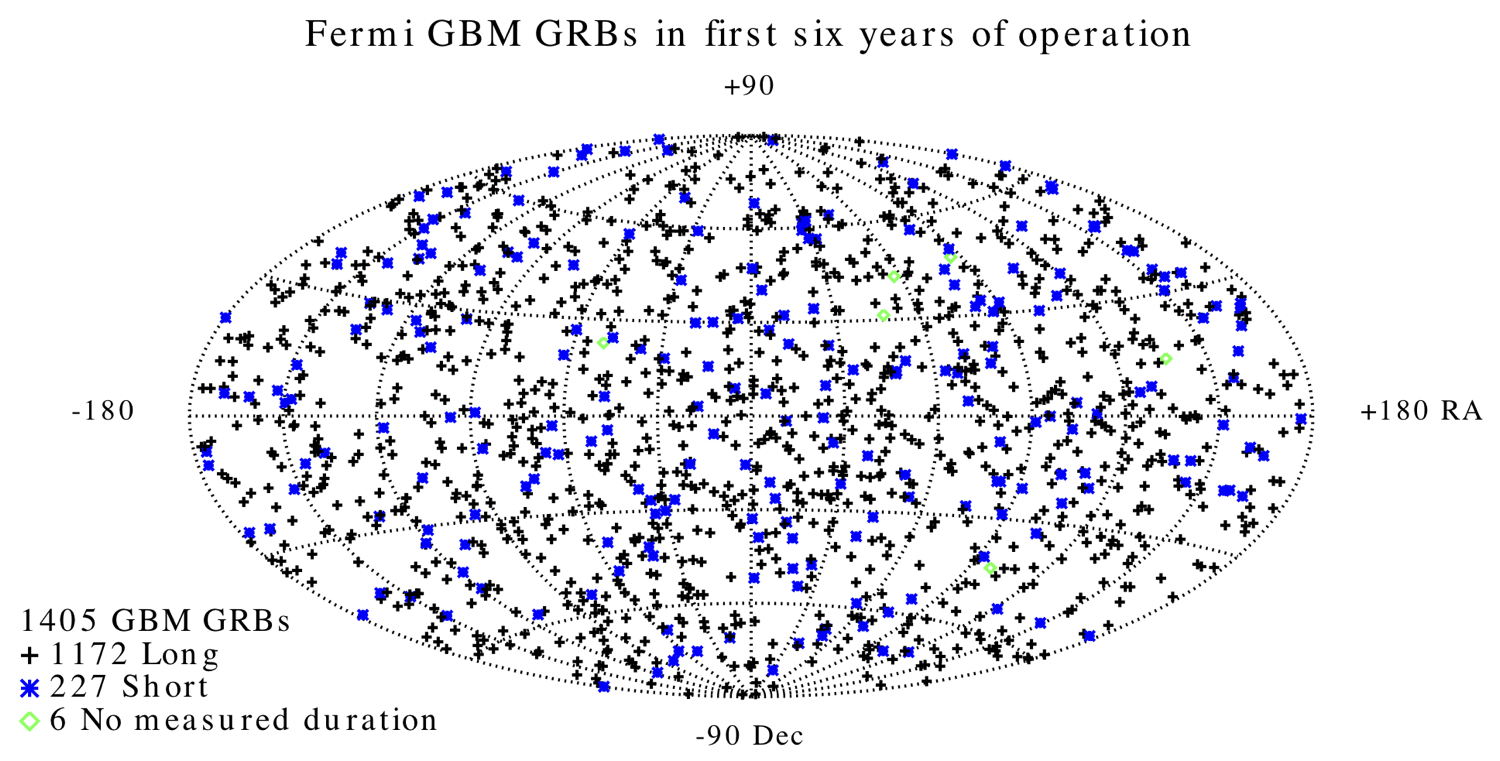
\includegraphics[width=0.9\linewidth]{figures/introduction/grbs.png}
\caption{The distribution of GRBs in the sky as observed by Fermi Gamma-ray Space Telescope in the first six years of operation shows that they are isotropically distributed and independent of their brightness, duration, spectrum, or any other characteristic. Credits to \cite{fermiwebsite}.}
\label{fig:grbs-localization}
\end{figure}
Gamma-ray bursts (GRBs) are among the most intense and energetic transients known to astronomers. They emit a vast amount of energy in a few seconds, equivalent to that emitted by a star like our Sun in its entire lifetime. Their origins have puzzled scientists since they were first serendipitously detected in the late 1960s by the Vela Satellite Network. Initially, it was believed that GRBs were of Galactic origin, but in the early 1990s, it was realized that they are isotropically distributed and have a cosmological origin \cite{mao_paczynski_1992}, \cite{meegan_fishman_wilson_1992}. \autoref{fig:grbs-localization} shows the distribution of GRBs in the sky as observed by Fermi Gamma-ray Space Telescope in the first six years of operation. Since the 1990s, GRBs have been the subject of intensive study, particularly after the Burst and Transient Source Experiment (BATSE) on board the Compton Gamma Ray Observatory began operations. The fluence, or energy per unit area, of a single GRB event ranges from $10^{-7}$ to $10^{-5} erg/cm^2$, and the isotropic energy, or the energy emitted in all directions, ranges from about $10^{48}$ to $10^{55} erg$. This makes GRBs the most violent and energetic event known to humankind \cite{Kumar_Zhang_2015}.
The nature of GRBs is still not fully understood, despite many years of research. The fireball model (represented in \autoref{fig:fireball}) is one historical model that explains the mechanism of GRBs. It proposes that they are produced by highly relativistic and collimated jets and that the interaction of blobs in the jet produces the prompt emission. In contrast, the interaction of the jet with ambient material produces the multiwavelength afterglow \cite{Bhat_2011}. GRBs are traditionally grouped into long (LGRBs) and short (SGRBs), depending on whether the burst lasts more or less than 2 s. In 1997, scientists discovered that long GRBs occur in star-forming regions. This led Paczynski to propose that core-collapse events cause LGRBs \cite{paczynski_1998}. Around the same time, MacFadyen and Woosley proposed the collapsar model, which states that a GRB is produced by a jet that emerges from the center of a collapsing star and penetrates the stellar envelope \cite{macfadyen_woosley_1999}. However, it wasn't until the discovery of \textit{SN2003dh} in association with \textit{GRB030329} that the link between GRBs and supernovae was confirmed \cite{hjorth_et_al_2003}. Since then, several other GRB-SN associations have been discovered, further solidifying the collapsar model as the explanation for LGRBs \cite{bromberg2012observational}. SGRBs are thought to be the result of compact binary mergers with at least one neutron star, such as a black hole and a neutron star (BH-NS), or two neutron stars (NS-NS) \cite{cohen1995distribution}, or two black holes (BH-BH) \cite{Perna_2016}. For this reason, they are also associated with 
gravitational wave (GW) counterparts \cite{abbott_et_al_2017}. The advanced Laser Interferometer Gravitational-Wave Observatory (LIGO) has detected several GWs, including \textit{GW150914}, \textit{GW151226}, \textit{GW170104}, and \textit{GW170817}. The observation of the association of \textit{GW170817} and \textit{GRB170817A} \cite{abbott_et_al_2017} confirms the NS-NS merger as a progenitor of SGRBs.
 \begin{figure}[t]
\centering
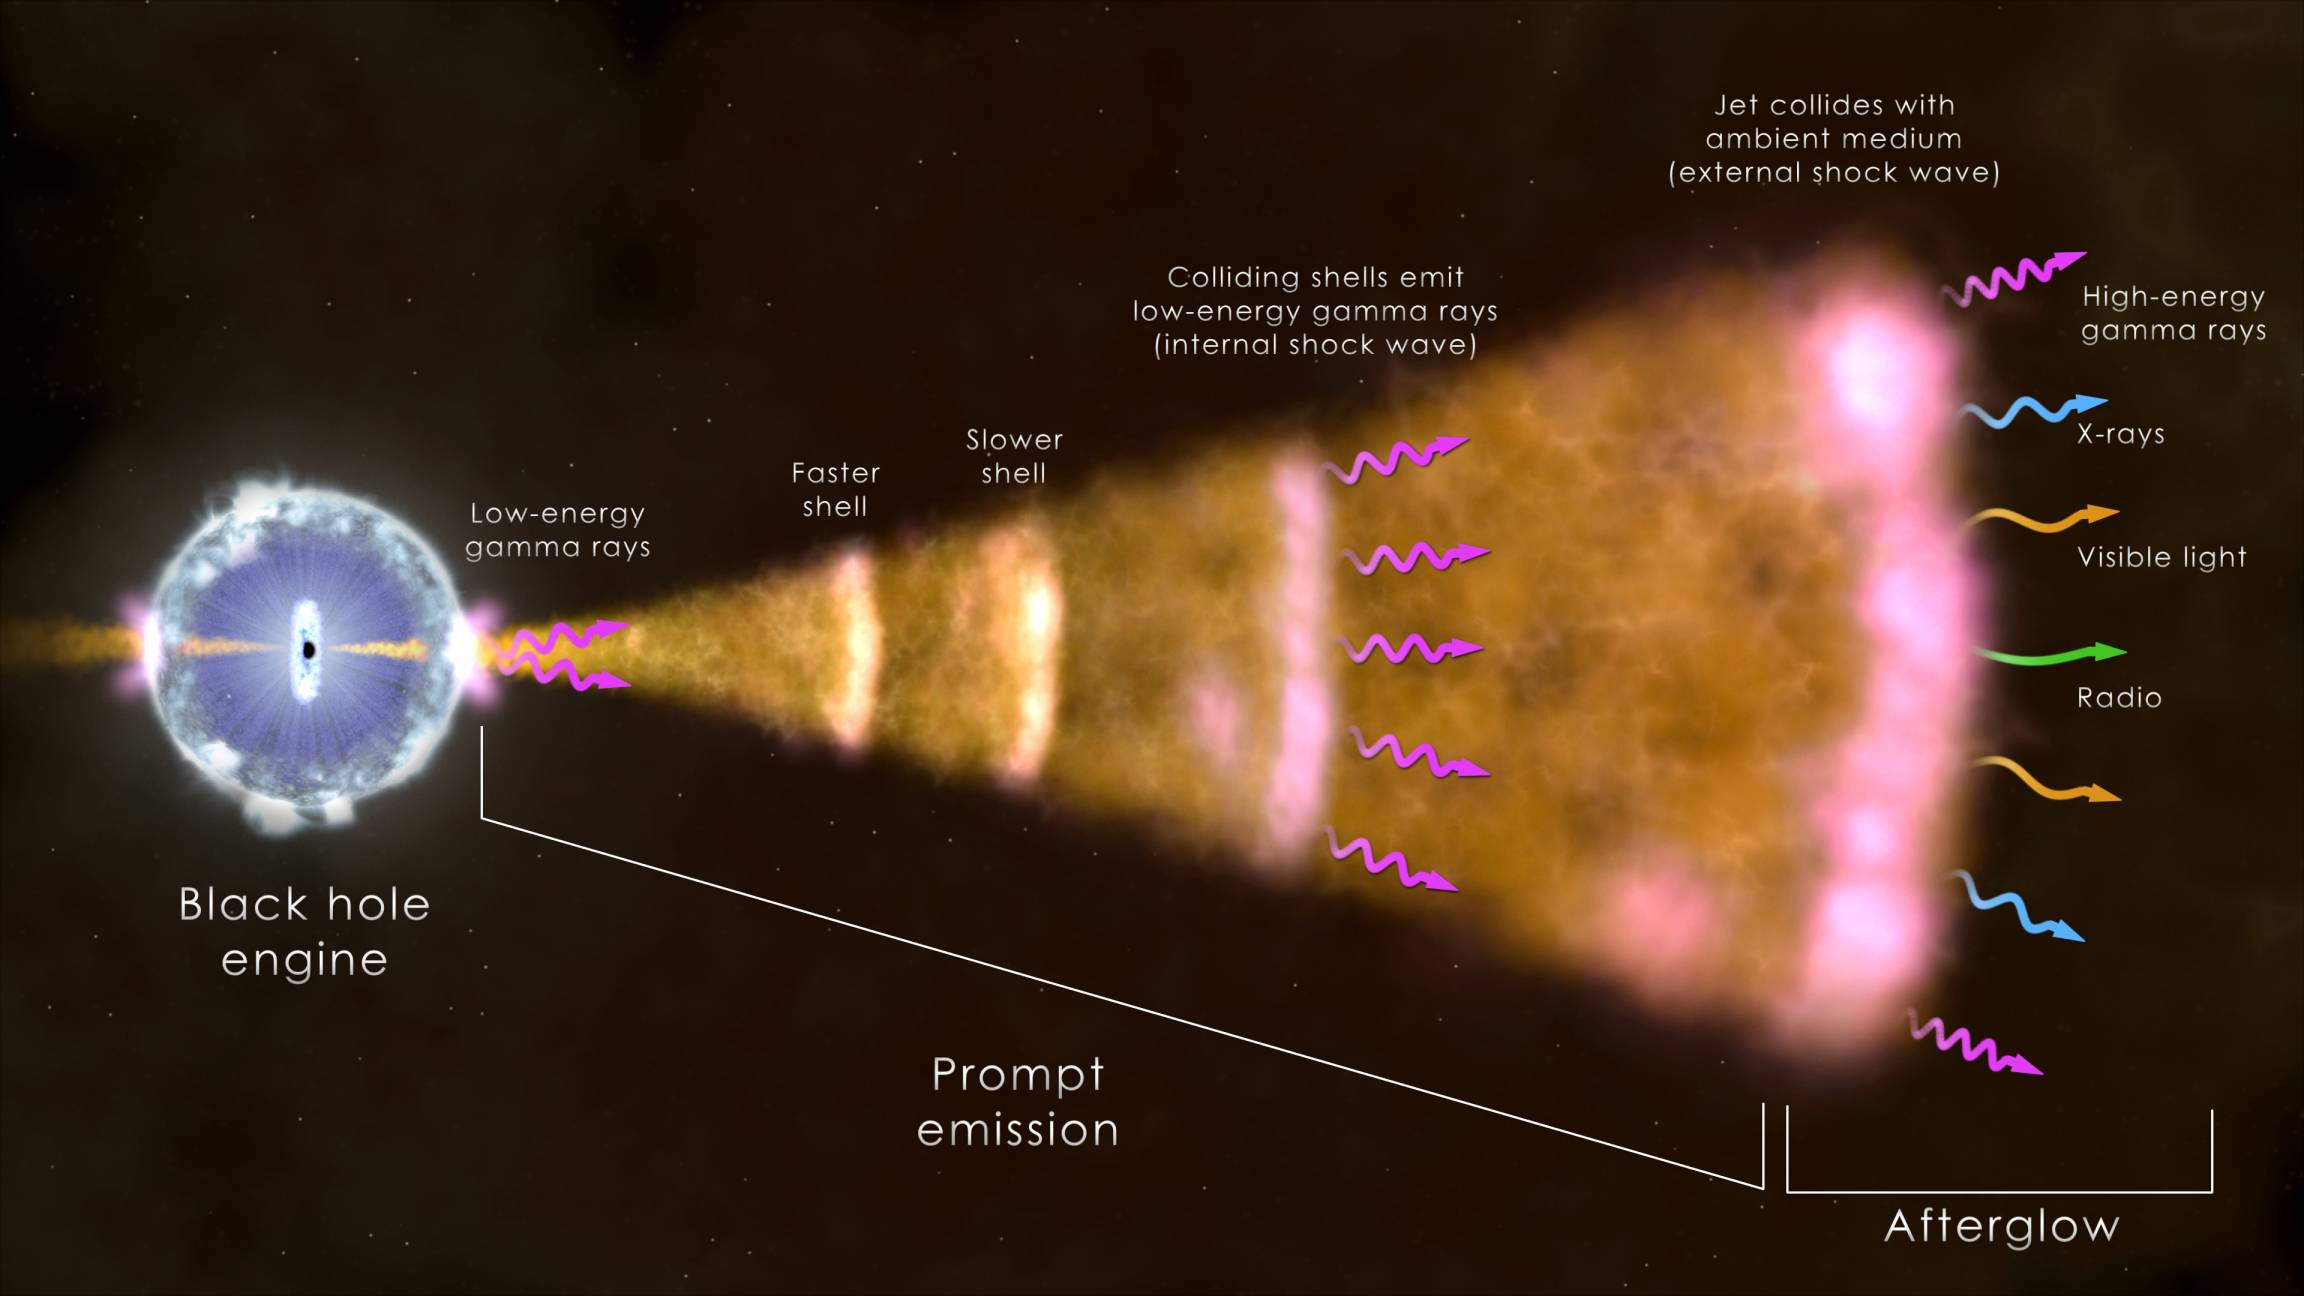
\includegraphics[width=0.9\linewidth]{figures/introduction/grb_fireball.jpg}
\caption{Sketch showing the different phases involved in the \textit{fireball} model with internal shocks producing the $\gamma$-ray prompt emission and external shock with the interstellar medium or the star wind responsible
for the afterglow phase observed in radio, optical, X-rays, and $\gamma$-rays. Credits to \cite{fermiwebsite}.}
\label{fig:fireball}
\end{figure}
